\subsection{Co-Saliency based Color Mapping}
\label{subsec:solver}
On the basis of the co-saliency model, we meet DR1 and DR2 in two ways: co-saliency based color assignment and co-saliency based palette generation.

\vspace{1.5mm}
\noindent\textbf{Co-saliency based Color Assignment}.
Given a good color palette with $P$ colors ($P\geq M$), the optimal color mapping can be obtained by
taking the co-saliency model in Eq.~\ref{eq:cosaliency} as the objective of the state-of-the-art color assignment method~\cite{Wang2018}. Starting from a random permutation of $P$ colors, we use the simulated annealing algorithm~\cite{aarts1989stochastic} to find the optimal permutation with two randomized strategies to improve the solution. One is randomly exchanging two colors from the selected $m$ colors and the other is replacing one color from the $m$ selected colors with the one chosen from the unselected $P-M$ colors. With a few iterations, we can obtain a reasonable color mapping as shown in Fig.~\ref{fig:teaser} bottom left.

\begin{figure}[h]
\centering
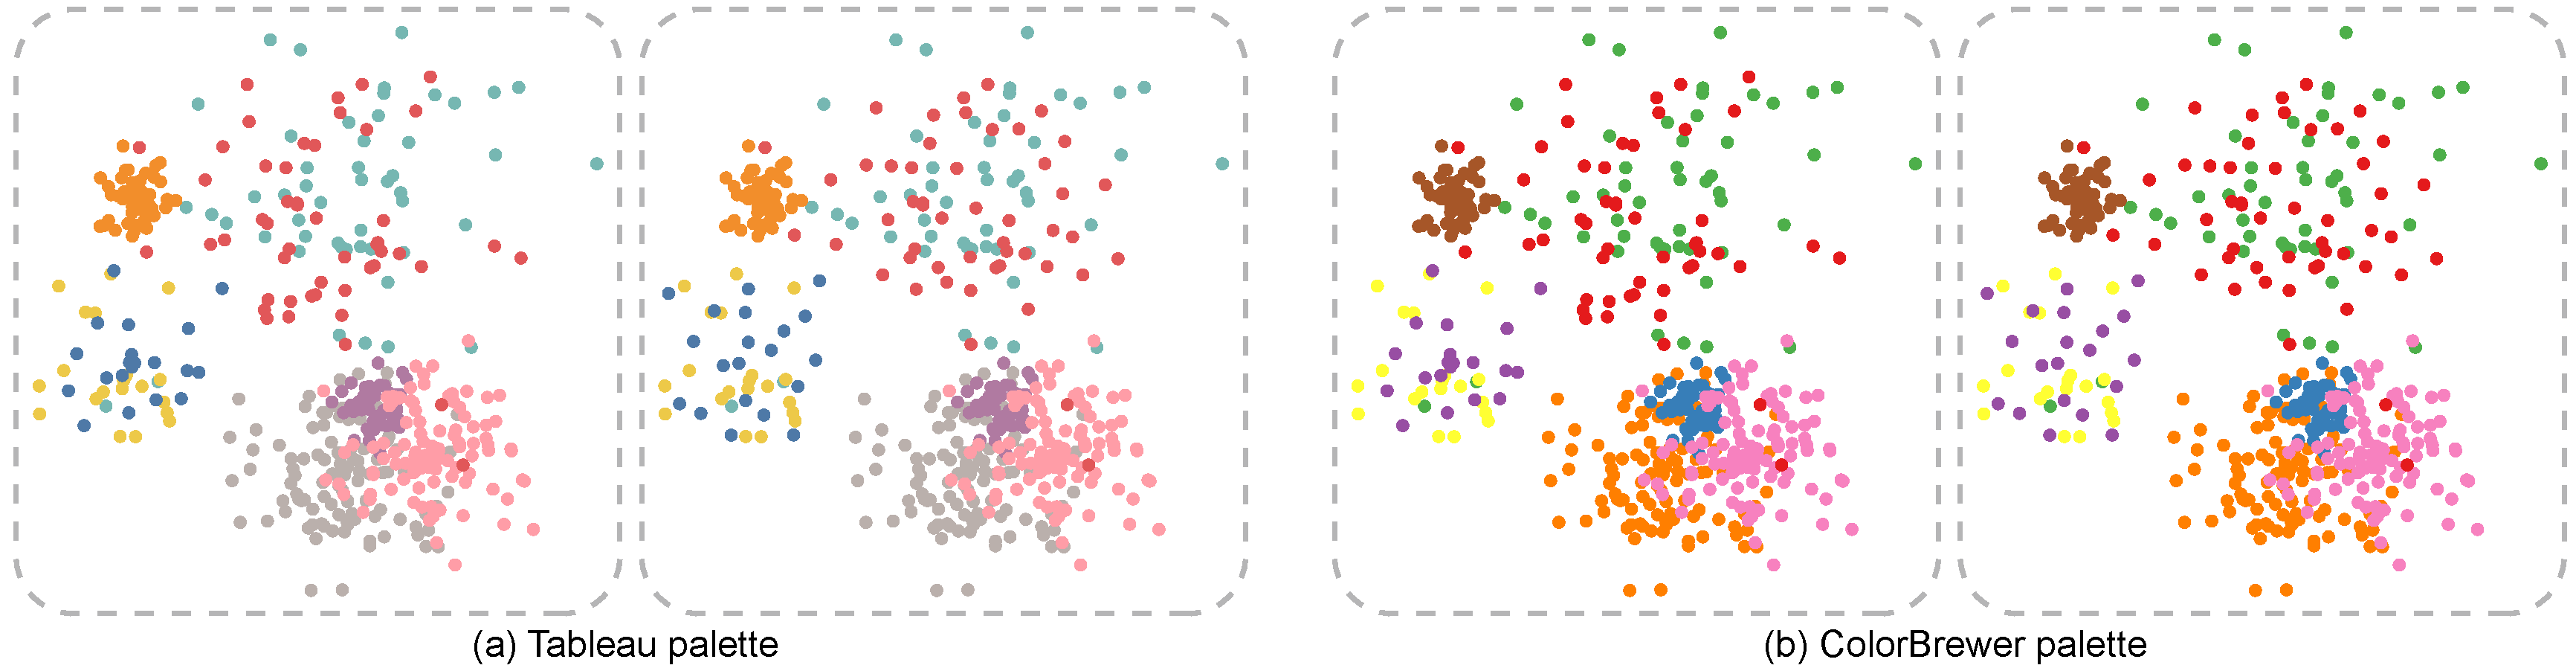
\includegraphics[width=.8\columnwidth]{figures/colorbrewer.pdf}
\caption{Visualizing the same data sets as shown in Fig.~\ref{fig:lambda} with the ColorBrewer palette and our assignment method.}
\vspace*{-3mm}
\label{fig:colorbrewer}
\end{figure}

However, this method has two major limitations: i) requiring users to try many palettes for selecting a good one; and ii) the design of most existing palettes is not oriented towards visual comparison so that even the best color assignment cannot provide prominent cues for this task.
%For example, all colors in the Tableau palette are highly discriminable and it is hardly to find a satisfactory solution, see Fig.~\ref{fig:teaser} (b). Thus, we prompt users to use our co-saliency based palette generation method.
For example, all colors in the ColorBrewer 8-class Set1~\cite{harrower2003colorbrewer} palette are highly discriminable, but it is hard to find a satisfactory solution. Fig.~\ref{fig:colorbrewer} shows an example, where the change of the red class is hard to identify at once even it is very distinctive. Since there exists other attractive colors, such as brown and blue. Thus, we prompt users to use our co-saliency based palette generation method.


\vspace{1.5mm}
\noindent\textbf{Co-saliency based Palette Generation}.
The recently proposed data-aware palette generation method~\cite{Lu21} automatically generates discriminable and preferable palettes by maximizing the combination of three palette quality measures: point distinctness, name difference, and color discrimination.
By replacing the first measure with our co-saliency model, the palette generation is formulated as an optimization problem:
\begin{equation}
\arg\max_{\mathbf{\tau}} E(\mathbf{\tau}) = \omega_0 E_{CoS} + \omega_1 E_{ND} + \omega_2 E_{CD}.
\label{eq:energyfunc}
\end{equation}
which consists of a co-saliency term $E_{CoS}$ (see Eq.~\ref{eq:cosaliency}), a name difference term $E_{ND}$ and a color discrimination term $E_{CD}$, balanced by $\omega_0$, $\omega_1$ and $\omega_2$. For more detail about $E_{ND}$ and $E_{CD}$, we refer readers to~\cite{Lu21}. By using the same optimization method as Lu et al.~\cite{Lu21}, we can generate desired colors in real time. %see Fig.~\ref{fig:teaser} (d).
For example, Fig.~\ref{fig:lambda}(b) shows an example which use same dataset within Fig.~\ref{fig:colorbrewer}, improves the distinctness of the two changed classes while maintains the class separability.



\subsection{Parameter Effect}
\label{subsec:parameter}
Besides different weights for different terms in palette generation~\cite{Lu21}, our co-saliency model involves three parameters: the weight $\lambda$ between two contrasts, the threshold for the class importance $\kappa$, and $\nu$ that is related to the definition of the class change degree which is used as our default class importance.
Since $\nu$ is fixed in our experiments and the class importance can be specified by user, we mainly discuss the effects of $\lambda$  and $\kappa$.

\begin{figure}[h]
\centering
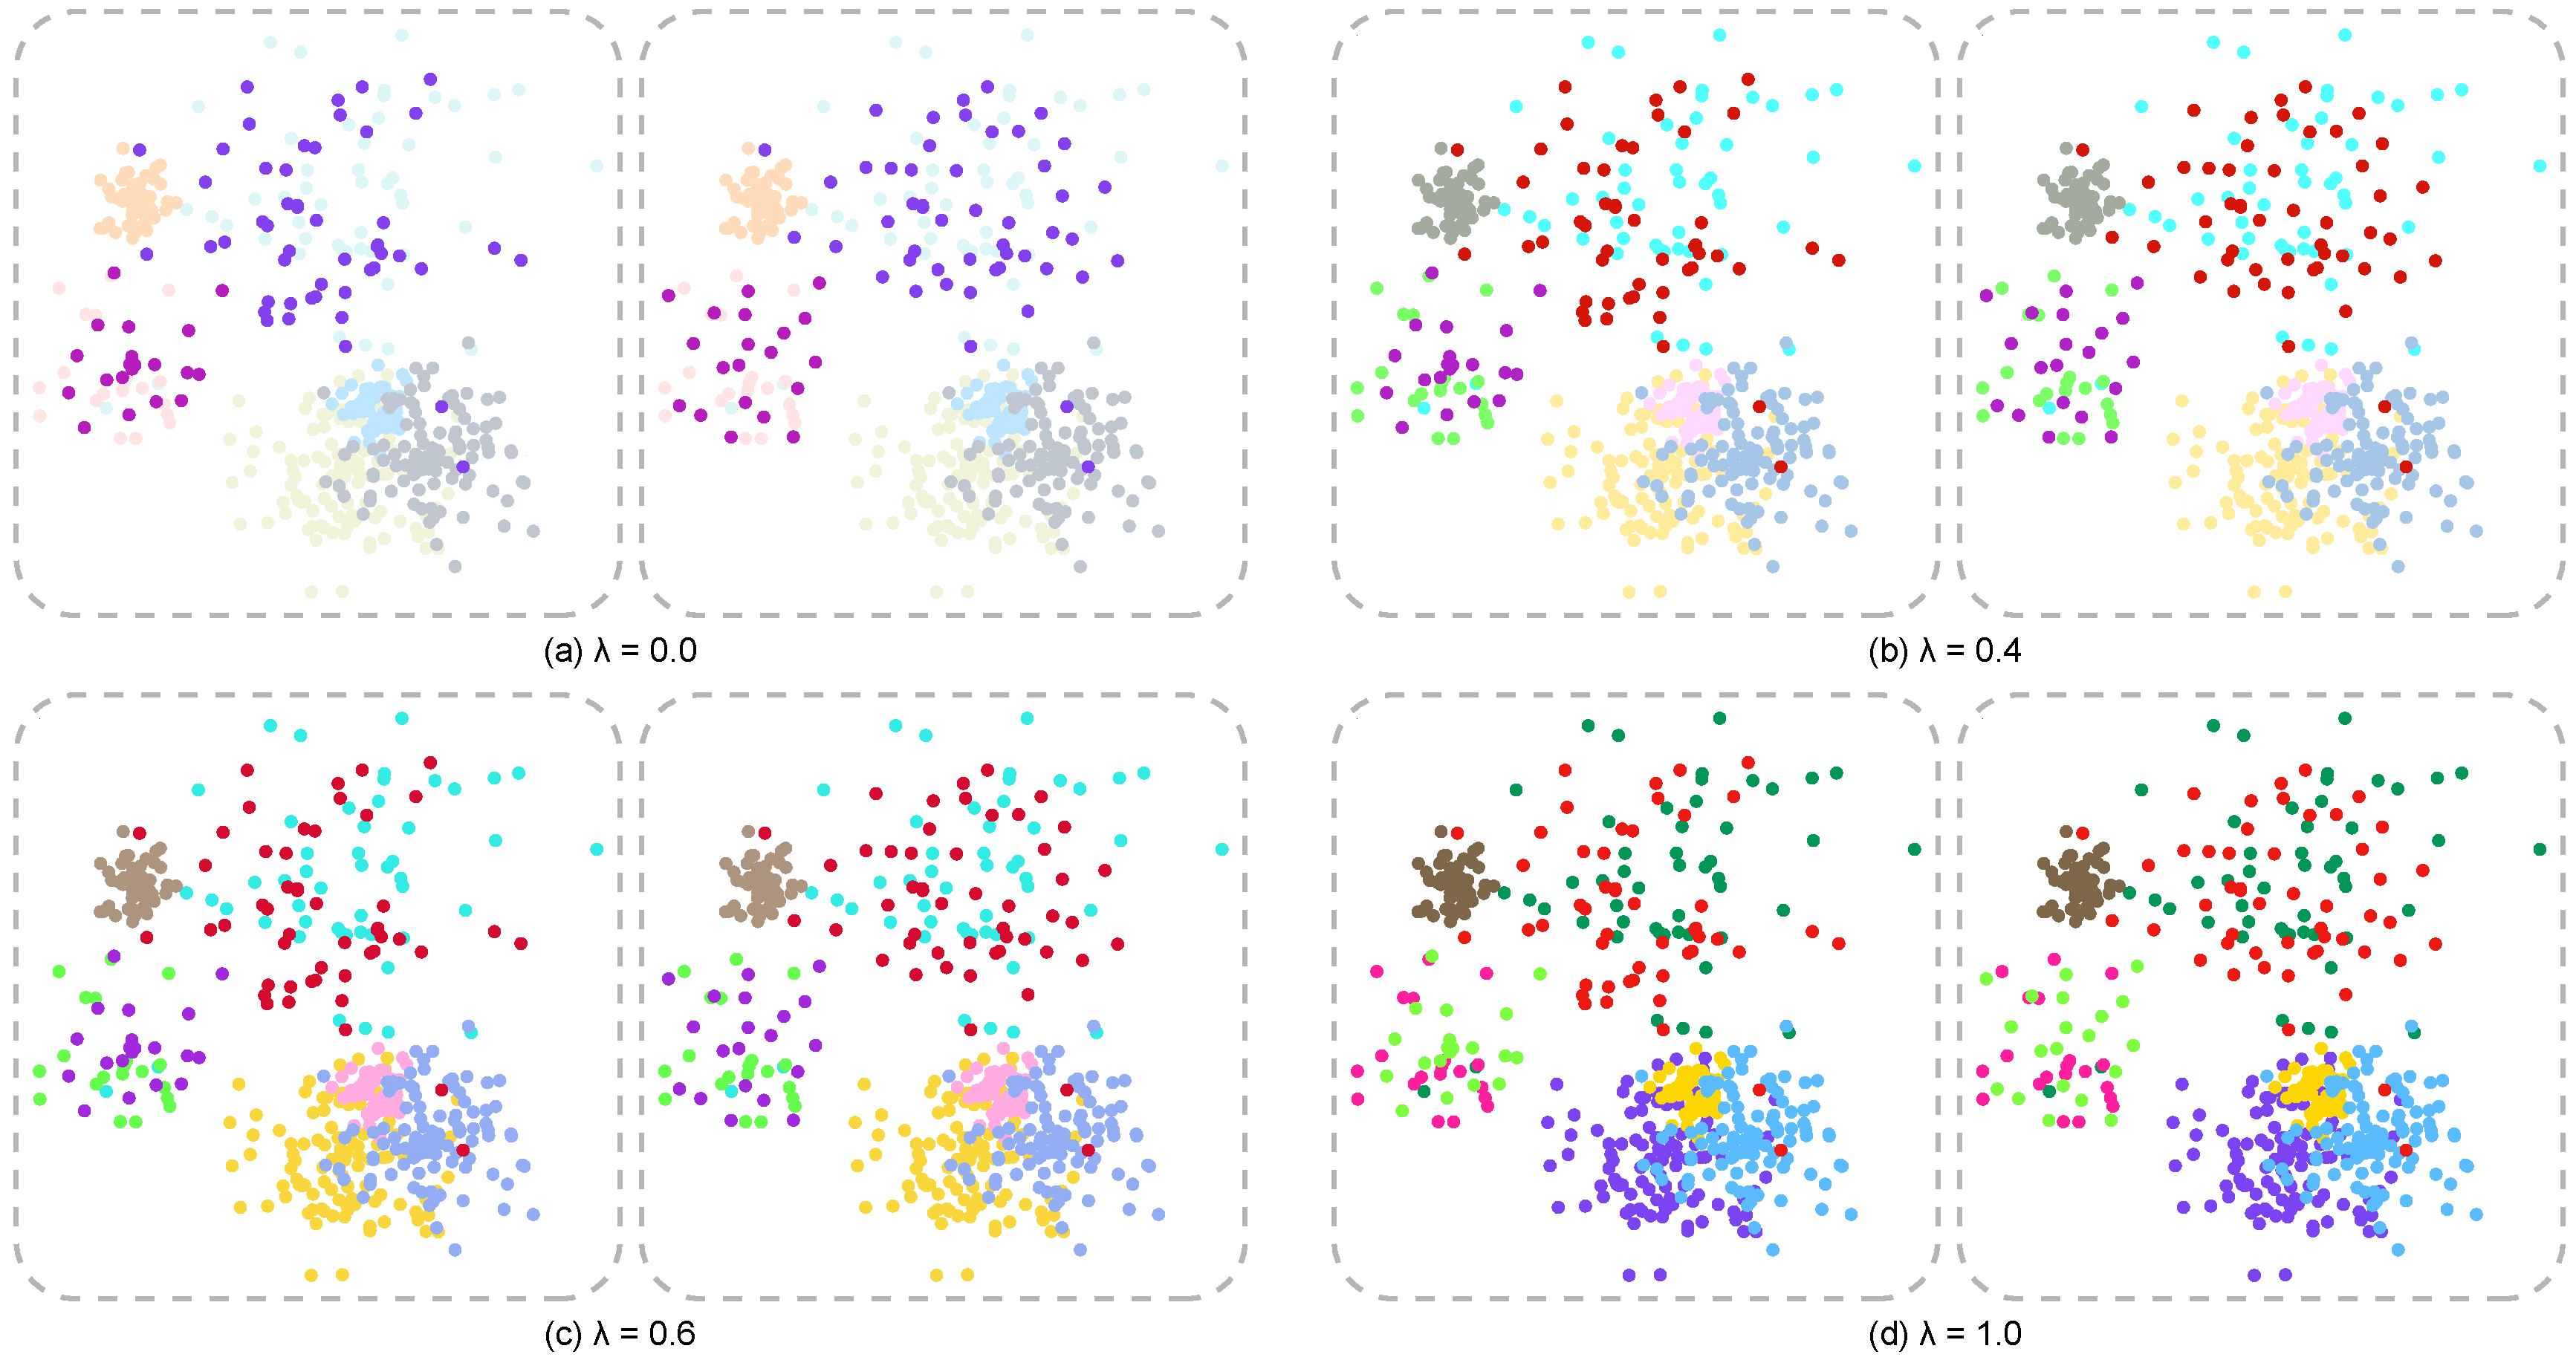
\includegraphics[width=0.8\textwidth]{figures/lambda.pdf}
\caption{Effect of $\lambda$: (a) result generated by only considering contrast to the background; (b) result generated by setting $\lambda$ to 0.4; (c) result generated by setting $\lambda$ to 0.6; (d) result generated by only considering contrast with nearest classes.}
\vspace*{-3mm}
\label{fig:lambda}
\end{figure}
%\vspace{3mm}

\noindent\textbf{Balancing Weight $\lambda$}.
Although this parameter modulates the influence between the class contrast with neighbors and background, it offers a compromise between DR1 and DR2.
As shown in Fig.~\ref{fig:lambda}(a), considering only the contrast to the background would have a good 'pop out' effect but other classes are hard to discriminate. While considering only the contrast with nearest neighbors, such as Fig.~\ref{fig:lambda}(d), all the classes are easy to distinguish but the changed classes are hard to find out.
This is reasonable, because pre-attentive vision
% processing mechanism
lets a bright saturated color region within  regions of de-saturated colors ``pop-out'' to the viewer~\cite{healey1995visualizing}.
In our experiments, we found that setting  $\lambda=0.4$ as the default allows to simultaneously emphasize changes and preserve the discriminability between classes, see an example in Fig.~\ref{fig:lambda}(b).


\vspace{1.5mm}
\noindent\textbf{Importance Threshold $\kappa$}.
The threshold $\kappa$ selects the classes with large importance to be highlighted.
With a default value of zero, all classes with importance value larger than zero are ensured to be highlighted. Likewise, a large $\kappa$ will de-emphasize classes with a small importance.
We further allow users to specify $\kappa$ by interaction through the control panel (see Sec.~\ref{sec:interaction}).

\begin{figure}[h]
\centering
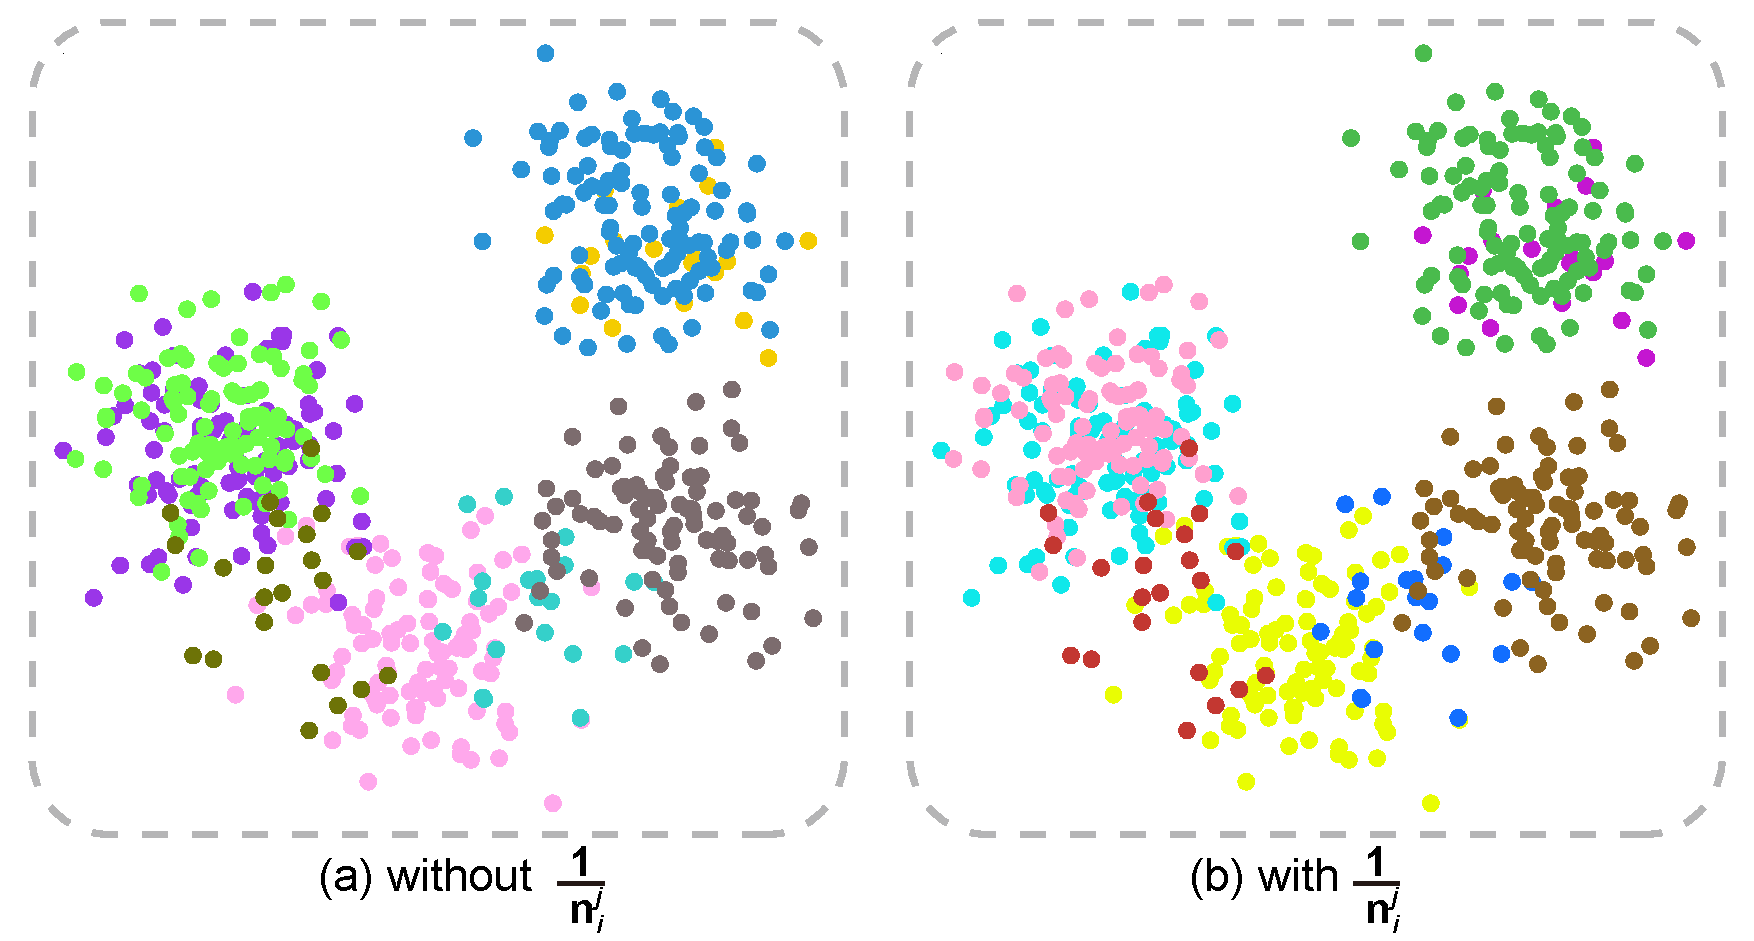
\includegraphics[width=0.8\textwidth]{figures/nij.pdf}
\caption{Effect of $\frac{1}{n^j_i}$: (a) without this term the small classes are hard to catch user's attention; (b) with this term, small classes are easy to find. Palettes are generated with same scatterplot.}
\vspace*{-3mm}
\label{fig:nij}
\end{figure}
%\vspace{.5em}

We can observe that when there's only one scatterplot and $\theta_i$ of each class is zero, then Equation.~\ref{eq:cosaliency} is very similar to the objective function of ~\cite{Wang2018}. Our method extends Wang et.al's work to multiple scatterplots with a carefully designed co-saliency model. Besides, we add $\frac{1}{n^j_i}$ to emphasize the class with less points. As shown in Fig.~\ref{fig:nij}(b), with this new term, the little classes, like red, blue and purple classes, become more discriminable.
